\documentclass[12pt,a4paper,oneside]{report}
\usepackage[utf8]{inputenc}
\usepackage[english,russian]{babel}
\usepackage{amsmath}
\usepackage{amssymb}
\usepackage{geometry}
\usepackage{sverb}
\usepackage{graphicx}
\usepackage{pdfpages}
\usepackage{url}
\usepackage{titlesec, blindtext, color}
\usepackage{listings}
\usepackage{pgfplots}
\pgfplotsset{compat=newest}
\graphicspath{{../}}
\DeclareGraphicsExtensions{.pdf,.png,.jpg}
\usepackage{tabularx}
\usepackage{subcaption}
\usepackage{colortbl}
\usepackage{multirow}
\usepackage{longtable}
\usepackage{enumitem}
\usepackage{algorithm}
\usepackage{tikz}
\usepackage[noend]{algpseudocode}
\usepackage{float}
\definecolor{gray75}{gray}{0.75}
\definecolor{Blue}{HTML}{5D8AA8}
\newcommand{\hsp}{\hspace{20pt}}

\newcommand{\RomanNumeralCaps}[1]
{\MakeUppercase{\romannumeral #1}}


% Для листинга кода:
\lstset{ %
	language=c,                 % выбор языка для подсветки (здесь это С)
	basicstyle=\small\sffamily, % размер и начертание шрифта для подсветки кода             % где поставить нумерацию строк (слева\справа)
	numberstyle=\tiny,           % размер шрифта для номеров строк
	stepnumber=1, 
	keywordstyle=\color{blue},% размер шага между двумя номерами строк
	numbersep=5pt,                % как далеко отстоят номера строк от подсвечиваемого кода
	showspaces=false,            % показывать или нет пробелы специальными отступами
	showstringspaces=false,      % показывать или нет пробелы в строках
	showtabs=false,             % показывать или нет табуляцию в строках
	frame=single,              % рисовать рамку вокруг кода
	tabsize=2,                 % размер табуляции по умолчанию равен 2 пробелам
	captionpos=t,              % позиция заголовка вверху [t] или внизу [b] 
	breaklines=true,           % автоматически переносить строки (да\нет)
	breakatwhitespace=false, % переносить строки только если есть пробел
	escapeinside={\#*}{*)}  % Стиль литералов
}


\titleformat{\chapter}[hang]{\Huge\bfseries}{\thechapter.\textcolor{gray75}\hsp}{0pt}{\Huge\bfseries}
\newcommand{\specchapter}[1]{\chapter*{#1}\addcontentsline{toc}{chapter}{#1}}
\newcommand{\specsection}[1]{\section*{#1}\addcontentsline{toc}{section}{#1}}
\newcommand{\specsubsection}[1]{\subsection*{#1}\addcontentsline{toc}{subsection}{#1}}

% геометрия


\setcounter{tocdepth}{4} % фикс переноса 
\righthyphenmin = 2
\tolerance = 2048


\thispagestyle{empty}

\geometry{pdftex, left = 3cm, right = 1cm, top = 2cm, bottom = 2cm}

\begin{document}


% геометрия


\setcounter{tocdepth}{4} % фикс переноса 
\righthyphenmin = 2
\tolerance = 2048


\thispagestyle{empty}

\thispagestyle{empty}
\noindent \begin{minipage}{0.15\textwidth}
	
\includegraphics[width=\linewidth]{b_logo}
\end{minipage}
\noindent\begin{minipage}{0.9\textwidth}\centering
	\textbf{Министерство науки и высшего образования Российской Федерации}\\
	\textbf{Федеральное государственное бюджетное образовательное учреждение высшего образования}\\
	\textbf{«Московский государственный технический университет имени Н.Э.~Баумана}\\
	\textbf{(национальный исследовательский университет)»}\\
	\textbf{(МГТУ им. Н.Э.~Баумана)}
\end{minipage}
\noindent\rule{18cm}{3pt}
\newline\newline
\noindent ФАКУЛЬТЕТ $\underline{\textbf{«ИНФОРМАТИКА И СИСТЕМЫ УПРАВЛЕНИЯ»}}$ \newline\newline
\noindent КАФЕДРА $\underline{\textbf{«ПРОГРАММНОЕ ОБЕСПЕЧЕНИЕ ЭВМ И ИНФОРМАЦИОННЫЕ}}$\newline\newline $\underline{\textbf{ТЕХНОЛОГИИ»(ИУ7)}}$\newline\newline
\noindent НАПРАВЛЕНИЕ ПОДГОТОВКИ $\underline{\textbf{09.03.04 ПРОГРАММНАЯ ИНЖЕНЕРИЯ}}$\newline\newline\newline\newline\newline\newline\newline
\begin{center}
    \begin{flushright}
    \Large\textbf{ОТЧЕТ}\newline
	\Large\textbf{по лабораторной работе № 2}\newline
	\end{flushright}
\end{center}
\noindent\textbf{Название:} $\underline{\text{Марковские процессы}}$\newline\newline
\noindent\textbf{Дисциплина:} $\underline{\text{Моделирование}}$\newline\newline\newline\newline\newline\newline\newline\newline
\begin{tabular}{lcp{5em}lp{2em}l}
	\noindent\textbf{Студент} &  $\underline{\text{ИУ7-71Б~~}}$ &             &\hspace{1cm} & & $\underline{\text{В.С.Плотников}}$ \\\cline{4-3}
	 & (Группа) & &(Подпись,дата)  & & (И.О.Фамилия) \\
	 & & & & &\\
	\noindent\textbf{Преподаватель} &  & &\hspace{1cm} & &$\underline{\text{И.В.Рудаков ~~~~}}$ \\\cline{4-3} 
	 &  & & (Подпись,дата)  & &(И.О.Фамилия) \\
    \end{tabular}
\begin{center}
	\vfill
	Москва, \the\year
\end{center}
\clearpage



\chapter{Задание лабораторной работы}
\quad Задача данной лабораторной работы для сложной системы S, имеющей не более 10 состояний, определить время нахождения системы в предельных состояниях, то есть при установившемся режиме работы.  

\chapter{Марковский процесс}
\quad Марковский процесс – случайный процесс, обладающий следующим свойством: для каждого момента времени  $t_{0}$ вероятность любого состояния  системы в будущем при t > $t_{0}$ зависит только от состояния системы в настоящем t = $t_{0}$ и не зависит от того, как процесс развивался в прошлом. 

Для Марковского процесса используются уравнения Колмогорова:
\begin{equation}
    F = (P'(t), P(t), \lambda)=0
\end{equation}
  где P(t) – вероятность, $\lambda$ – набор коэффициентов.
  
Вероятностью i-ого состояния называется вероятность $P_{i}(t)$ того, что в момент времени t система будет находиться в состоянии $S_{i}$. Для любого момента t сумма вероятностей всех состояний равна единице.

Для нахождения предельных вероятностей системы $S_{n}$ следующего вида:
\begin{figure}[H]
	\centering
	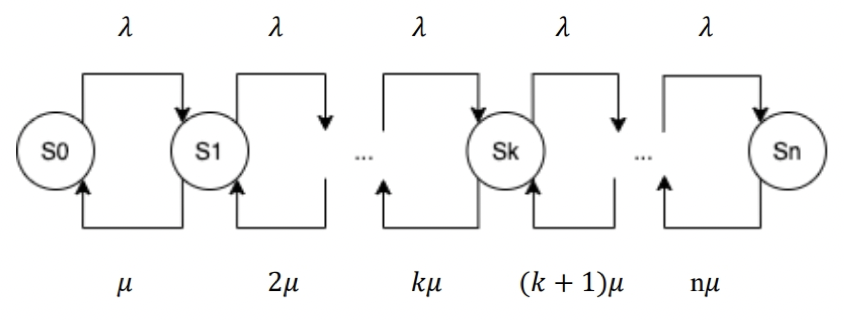
\includegraphics[scale=0.4]{1.png}
	\label{fig:screenshot001}
	\caption{Граф состояний}
\end{figure}

Используется система уравнений:
\begin{figure}[H]
	\centering
	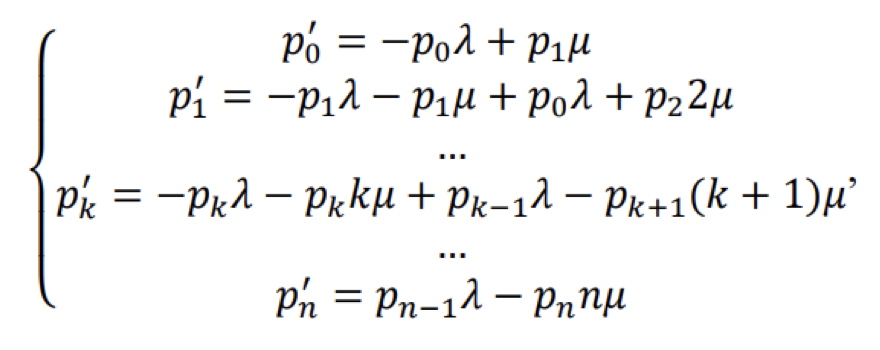
\includegraphics[scale=0.3]{2.png}
	\label{fig:screenshot002}
	\caption{Система уравнения Колмогорова}
\end{figure}
где каждое уравнение составляется по следующему принципу: в левой части каждого уравнения стоит производная вероятности состояния, а правая содержит столько членов, сколько стрелок связано с данным состоянием. Если стрелка направлена “из” состояния, соответствующий член имеет знак “–”, если “в” состояние, то знак “+”. Каждый член равен произведению плотности вероятности перехода (интенсивности), соответствующий данной стрелке, и вероятности того состояния, из которого выходит стрелка.

\chapter{Результаты работы}
На рисунках \ref{fig:screenshot003} и \ref{fig:screenshot004} показаны примеры для систем, состоящих из 5 и 10 состояний.
\begin{figure}[h]
	\centering
	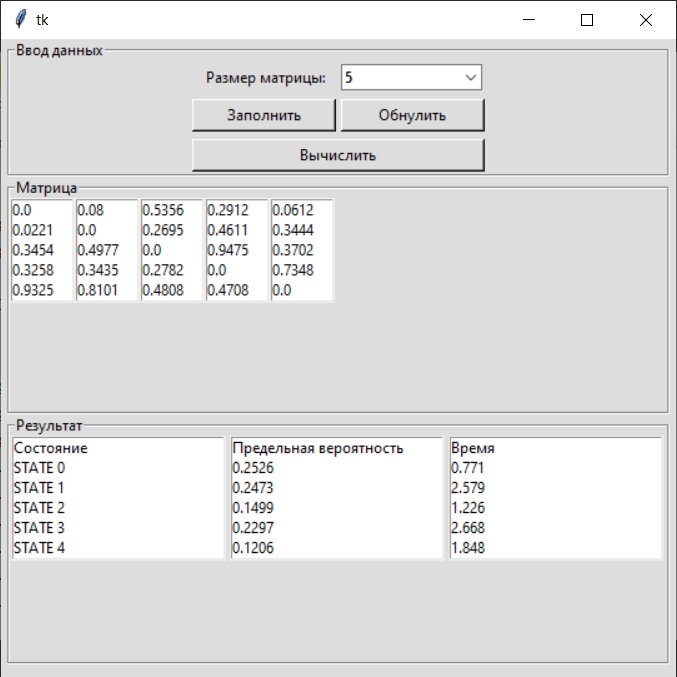
\includegraphics[scale=0.59]{4.png}
	\caption{Система из 5 состояний}
	\label{fig:screenshot003}
	
\end{figure}

\begin{figure}[h]
	\centering
	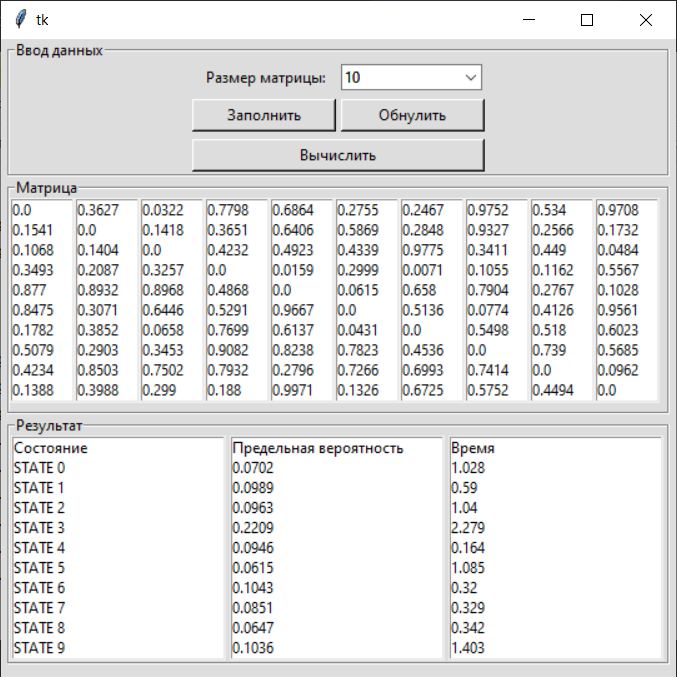
\includegraphics[scale=0.59]{3.png}
	\caption{Система из 10 состояний}
	\label{fig:screenshot004}
	
\end{figure}
\end{document}

